Um dem Benutzer den Einstieg zur Verwendung des Paketes zu erleichtern, sind in den folgenden Kapiteln Beispiele und genaue Erklärungen zu allen wichtigen Funktionen. Dabei werden in Kapitel \ref{sec:example_createHelpers} alle wichtigen Variablen erstellt, die dann in den Kapiteln \ref{sec:example_withPunctuation} und \ref{sec:example_withoutPunctuation} beim Kodieren und Dekodieren verwendet werden. Zum Schluss werden in Kapitel \ref{sec:example_simulations} die verschiedenen Möglichkeiten der Ausführung von Simulationen erläutert.

\section{Erzeugen von Kodierer, Permutationsvektor und Punktierungsmatrix}
\label{sec:example_createHelpers}
Zuerst werden Hilfsvariablen erzeugt, die für die folgende Kodierungs- und Dekodierungsverfahren benötigt werden. Diese Variablen müssen nicht unbedingt mitgegebenen werden, dann werden die Standard-Werte verwendet. Das bedeutet, dass falls keine Punktierungsmatrix übergeben wird, der Standard-Wert \texttt{NULL} ist und darum nicht punktiert wird. Ebenfalls wird nicht permutiert, wenn kein Permutationsvektor als Argument übergeben wird. Es wird zwar ein Permutationsvektor benötigt, damit die Interleaver richtig arbeiten können, jedoch wird ein Vektor vom Typ \texttt{PRIMITIVE} verwendet, dieser allerdings ändert die Reihenfolge der Bits nicht (root=0). Beim Kodierer verhält es sich ähnlich, jedoch wird hier ein vordefinierter Standard-Faltungskodierer verwendet (\texttt{ConvGenerateRscEncoder(2,2,c(5,7))}), dieser wird in allen Turbo-Kode-Funktionen benützt, falls kein eigener Kodierer übergeben wird.

\begin{lstlisting}[caption=Erzeugung von Kodierer und Punktierungsmatrix, label={lst:createHelpersCoderPunctuation}, float=!ht]
input <- c(1,0,1,1,0)

coder <- ConvGenerateEncoder(2, 2, c(4,5))

punctuation.matrix <- TurboGetPunctuationMatrix(c(1,1,0))
\end{lstlisting}

Wie im Listing \ref{lst:createHelpersCoderPunctuation} zu sehen ist, wird als allererstes eine zu kodierende Nachricht erzeugt. Danach kann eine Punktierungsmatrix, mithilfe der oben dargestellt Funktion erstellt werden. Anschließend wird ein nicht rekursiver Faltungskodierer, mit der Funktion vom Faltungskode-Teil des Paketes \cite{nocker}, erzeugt. Dabei wurde ein Kodierer mit zwei Registern und zwei Ausgängen gewählt. Wichtig ist, dass der erste Ausgang vom Eingang durchgeschalten wird damit es ein systematischer Kodierer ist. Das wird erreicht, indem das erste Generatorpolynom mit $2^M = 2^2 = 4$ deklariert wird. Zum Schluss wird noch eine Punktierungsmatrix erstellt, die aus nur einer Spalte besteht und jedes dritte Bit aus dem Vektor entfernt. Bei einer 1 wird das Bit behalten, bei einer 0 verworfen.

\begin{lstlisting}[caption=Erzeugung von verschiedenen Permutationsvektoren, label={lst:createHelpersPermutation}, float=!ht]
permutation.vector.random <- TurboGetPermutation(length(input), coder, "RANDOM")
permutation.vector.primitve <- TurboGetPermutation(length(input), coder, "PRIMITIVE", list(root=3))

input2 <- c(1,0,1,1,0,1)
permutation.vector.cyclic <- TurboGetPermutation(length(input2), coder, "CYCLIC", list(cols=4, rows=2, distance=2))
permutation.vector.block <- TurboGetPermutation(length(input2), coder, "BLOCK", list(cols=4, rows=2))
permutation.vector.helical <- TurboGetPermutation(length(input2), coder, "HELICAL", list(cols=4, rows=2))
permutation.vector.diagonal <- TurboGetPermutation(length(input2), coder, "DIAGONAL", list(cols=4, rows=2))
\end{lstlisting}

Als nächstes benötigt der Benutzer noch einen Permutationsvektor, dieser wird im Listing \ref{lst:createHelpersPermutation} erzeugt. Dafür ist die erzeugte Nachricht nötig, da die Länge als Eingabeparameter nötig ist. Dabei wird jeder Typ einmal verwendet. Bei den ersten beiden werden die Eingangsbits von Listing \ref{lst:createHelpersCoderPunctuation} benützt. Da bei den restlichen Typen eine Matrix benötigt wird, muss die Länge der Eingangsbits genau in einer Matrix Platz finden, deshalb wurde ein zweiter Eingangsvektor definiert, der allerdings nur als Demonstration für die anderen Permutationstypen dienen sollte, dieser wird in den weiteren Beispielen nicht weiter verwendet.

\section{Kodieren und Dekodieren ohne Punktierung}
\label{sec:example_withoutPunctuation}
Nachdem alle benötigten Variablen gesetzt wurden kann nun die Kodierung und Dekodierung vorgenommen werden. Dabei wird zuerst ohne Punktierung gearbeitet, jedoch alle anderen zuvor definierten Variablen verwendet.

\begin{lstlisting}[caption=Kodierung und Dekodierung ohne Punktierung, label={lst:encodeDecodeWithoutPunctuation}, float=!ht]
encoded <- TurboEncode(input, permutation.vector.random, coder, parity.index = 2)
encoded
[1] -1 -1 -1  1  1  1 -1  1  1 -1 -1  1  1 -1 -1  1 -1 -1  1  1  1

encoded.noisy <- ApplyNoise(encoded, SNR.db = 0.1)
round(encoded.noisy, 2)
[1] -2.41 -2.36 -0.26  1.06  1.37  0.22  1.13  0.93  0.33 -1.15 -1.18  0.59
[13]  1.32 -0.31 -1.37 -0.01 -1.42 -1.62  2.18  2.29  0.93

decoded <- TurboDecode(encoded.noisy, permutation.vector.random, iterations = 5, coder, parity.index = 2)
decoded
$output.soft
[1]  -1.394185  1.394185  2.775904 -1.394185  2.775904

$output.hard
[1] 1 0 1 1 0
\end{lstlisting}

Der gesamte Vorgang lässt sich in wenigen Zeilen erledigen, wie in Listing \ref{lst:encodeDecodeWithoutPunctuation} zu sehen ist. Zuerst werden einfach die zuvor definierten Variablen der Kodierungsfunktion mitgegeben, als letzter Parameter wird noch der Index des zu verwendeten Ausgangs des Kodierers angegeben (zwei in diesem Fall). Danach erhält man das kodierte Signal mit dem Signalpegel 1 und -1. Dieses Signal wird dann einem Signal/Rausch-Verhältnis von 0.1dB  verrauscht und anschließend ausgegeben, damit man den Unterschied zwischen Originalsignal und Verrauschtem sieht. Dabei werden nur zwei Nachkommastellen ausgegeben, um die Länge der Ausgabe zu kürzen. 

Nachdem das Signal kodiert und übertragen wurde, kann der Empfänger es nun wieder dekodieren. Dabei schickt er das empfangene Signal in die Dekodierungsfunktion, als Iterationsanzahl wird fünf gewählt. Das Ergebnis ist dann eine Liste mit den Soft- und Hard-Werten. Dabei ist zu erkennen, dass positive Soft-Werte auf eine 0 und negative auf eine 1 abgebildet werden. Bei diesem Beispiel ist schön zu sehen, dass auch ein ziemlich verrauschtes Signal vom Turbo-Dekodierer wieder hergestellt werden kann.
\section{Kodieren und Dekodieren mit Punktierung}
\label{sec:example_withPunctuation}

Der gleiche Ablauf kann mit Punktierung wiederholt werden. Dabei werden am Ende des Kodierungsvorgangs die Bits entfernt, bei denen in der Matrix eine 0 steht und die Bits durchgelassen bei denen eine 1 steht. Beim Dekodierungsvorgang wird an den Stellen eine 0 eingefügt, die zuvor entfernt wurden. Da der Signalpegel normalerweise -1 oder 1 ist, wird für die wieder eingefügten Bits eine 0 eingefügt, da unklar ist welche Signalpegel sie tatsächlich haben. Mit einer 0 besteht die gleiche Wahrscheinlichkeit für eine -1 oder 1 an dieser Stelle.

\begin{lstlisting}[caption=Kodierung und Dekodierung mit Punktierung, label={lst:encodeDecodeWithPunctuation}, float=!ht]
encoded.punctured <- TurboEncode(input, permutation.vector.random, coder, parity.index = 2, punctuation.matrix)
encoded.punctured
$original
[1] -1 -1 -1  1  1  1 -1  1  1 -1 -1  1  1 -1 -1  1 -1 -1  1  1  1

$punctured
[1] -1 -1  1  1 -1  1 -1 -1  1 -1  1 -1  1  1

decoded.punctured <- TurboDecode(encoded.punctured$punctured, permutation.vector.random, iterations = 5, coder, parity.index = 2, punctuation.matrix)
decoded.punctured
$output.soft
[1] -6  6 -6 -6  6

$output.hard
[1] 1 0 1 1 0
\end{lstlisting}

Im dargestellten Listing \ref{lst:encodeDecodeWithPunctuation} sieht man nun das Verfahren mit Punktierung. Dort wird als erstes der Kodierfunktion die Punktierungsmatrix mitgegeben. Dadurch werden Bits entfernt, wie man an der Ausgabe sieht. Zurückgeliefert wird eine Liste mit dem Originalvektor ohne Punktierung und einmal der Punktierte, das muss bei der Verwendung dieser Variable bedacht werden. Der Dekodierfunktion wird nun das punktierte Signal mitgegeben und die fügt als erstes die gelöschten Bits wieder ein und dekodiert das Signal dann. Als Resultat bekommt man wieder eine Liste die Soft- und Hard-Werte enthalten. Das Ergebnis nach fünf Iterationen stimmt mit der Ausgangsnachricht überein, somit war die Dekodierung erfolgreich.

\section{Simulationen}
\label{sec:example_simulations}

Die nächsten drei Unterkapitel werden sich den verschiedenen Simulationsfunktionen im Paket beschäftigen. Dabei wird zuerst eine reine Simulation des Turbo-Kode-Verfahrens vorgenommen. Im Anschluss werden alle drei Kanalkodierungsverfahren (Block-, Faltungs und Turbo-Kodes) miteinander verglichen und zum Schluss wird noch die Hilfsfunktion zur Darstellung verschiedener Simulationsergebnisse an einem Beispiel erklärt.

\subsection{Turbo-Kode}
\label{sec:example_simulations_turbo}

Im folgenden Beispiel wird eine Simulation des Turbo-Kode-Verfahren durchgeführt, bei der alle Parameter bestimmt werden können, wie Permutationstyp, Länge der Nachricht, Kodierer, zu testende Signal/Rausch-Verhältnisse, Anzahl von Dekodierungsiterationen und Anzahl der Wiederholungen. Als Ergebnis wird ein Dataframe zurückgegeben, das die Bitfehlerrate für jedes Signal/Rausch-Verhältnis beinhaltet.

\begin{lstlisting}[caption=Turbo-Kode-Simulation, label={lst:turboCodeSimulation}, float=!ht]
df1 <- TurboSimulation(coder, "DIAGONAL", list(rows=2,cols=501), decode.iterations = 3, msg.length = 1000, min.db = 0.01, max.db = 0.1, db.interval = 0.01, iterations.per.db = 50, punctuation.matrix)
df1
     db     ber
1  0.01 0.11294
2  0.02 0.11430
3  0.03 0.11238
4  0.04 0.11208
5  0.05 0.11050
6  0.06 0.10880
7  0.07 0.10832
8  0.08 0.10784
9  0.09 0.10868
10 0.10 0.10720
\end{lstlisting}

In Listing \ref{lst:turboCodeSimulation} wurde eine Nachrichtenlänge von 1000 Bits gewählt, die zwischen 0.01-0.1dB bei drei Dekodierungsiterationen getestet werden. Nach 50 Durchläufen wird der Mittelwert gebildet und in das zurückgegebene Dataframe geschrieben. Dieses kann entweder im Visualisierungsbericht dargestellt werden (\texttt{visualize=TRUE}), oder mit der in Kapitel \ref{sec:example_simulations_plot} vorgestellten Funktion.

\subsection{Kanalkodierung}
\label{sec:example_simulations_channel}

Damit ein Vergleich der drei Kanalkodierungsverfahren möglich ist, müssen alle drei Verfahren mit den gleichen Parameter getestet werden. Danach kann mittels der Bitfehlerrate ein genauer Vergleich angestellt werden und die Vor- und Nachteile der Verfahren analysiert werden.

\begin{lstlisting}[caption=Kanalkodierungs-Simulation, label={lst:channelCodeSimulation}, float=!ht]
ChannelcodingSimulation(msg.length = 50, max.db = 1, turbo.decode.iterations = 3)
    db block.ber   conv.ber  turbo.ber
1  0.1 0.1911429 0.05800000 0.06085714
2  0.2 0.1802857 0.06857143 0.05485714
3  0.3 0.2011429 0.06714286 0.05171429
4  0.4 0.1862857 0.06171429 0.03085714
5  0.5 0.1840000 0.04342857 0.03657143
6  0.6 0.1745714 0.06485714 0.03200000
7  0.7 0.1697143 0.05085714 0.03428571
8  0.8 0.1577143 0.03485714 0.02342857
9  0.9 0.1668571 0.04285714 0.02285714
10 1.0 0.1442857 0.03342857 0.01457143
\end{lstlisting}

Bei dem Beispiel in Listing \ref{lst:channelCodeSimulation} wurde eine Nachrichtenlänge von 50 Bits gewählt, die bis maximal 1dB Signal/Rausch-Verhältnis getestet wird und drei Dekodierungsiterationen im Turbo-Dekodierer vorgenommen werden. Bei allen anderen Parameter wurden die Standard-Werte verwendet. Das Ergebnis ist ein Dataframe, das für jedes einzelne Verfahren eine Spalte mit den zugehörigen Bitfehlerraten enthält. Der direkte Vergleich in einer Grafik ist im Visualisierungsbericht enthalten (\texttt{visualize=TRUE}). 

\subsection{Vergleich mehrerer Simulationen}
\label{sec:example_simulations_plot}

Nachdem die reinen Dataframes als Rückgabewert der Simulation von Kapitel \ref{sec:example_simulations_turbo} nicht wirklich aussagekräftig sein, ermöglicht die folgende Funktion eine Darstellung verschiedener Simulationen in einer Grafik. Dadurch lassen sich diese miteinander besser vergleiche und genaue Analysen sind möglich.

\begin{lstlisting}[caption=Vergleich mehrerer Simulationen, label={lst:plotSimulations}, float=!ht]
df2 <- TurboSimulation(msg.length = 1000, min.db = 0.01, max.db = 0.1, db.interval = 0.01)

PlotSimulationData(df1, df2)
\end{lstlisting}

\begin{figure}[ht]
\centering
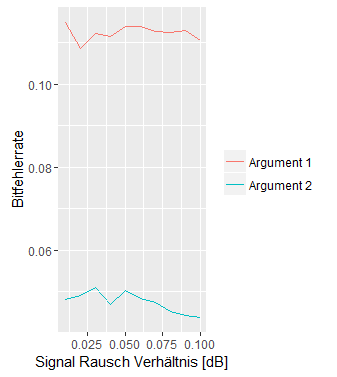
\includegraphics[width=\ScaleIfNeeded]{pictures/PlotSimulations}
\caption{Vergleich zweier Simulationen}
\label{pic:plotSimulations}
\end{figure}

Im Listing \ref{lst:plotSimulations} werden zwei verschiedene Simulationen mit unterschiedlichen Kodierern miteinander verglichen. Die erste Simulation stammt noch von Kapitel \ref{sec:example_simulations_turbo}, diese wird mit der Simulation des Standard-Kodierers verglichen. Die erstellte Grafik ist in Abbildung \ref{pic:plotSimulations} zu sehen, da ist deutlich zu erkennen, dass die erste Simulation klar die besseren Ergebnisse liefert.